%%==========================================================================
\section{Experiments}
\label{sec:experiments}

We have used synthetically generated data as well as real captured data to evaluate the SuperMatching algorithm.
To demonstrate that the SuperMatching algorithm is independent of feature descriptors, several descriptors have been used.
For 2D deformable surfaces,
%%%RRM unclear. do you mean 2D images of deforming 3D surfaces
SIFT features~\cite{Lowe04} were used.
To test 3D surface matching (without color information), slippage features~\cite{Bokeloh08} were employed.
For 3D coloured shapes, both SIFT and slippage features were employed.
We used third-order matching in our experiments, and note it would be simple to use higher order.
%%%RRM But presumably slower?
%For greater than third higher-order, it is easy to replace the potential by relevant polygonal definitions.

%%%RRM I can see a couple of problems with the experiments section as it stands
%%%RRM (i) the releveance of the experiments in 5.1 is not so clear.
%%%RRM 5.1 is a computer vision style problem, not graphics.
%%%RRM (ii) Each experiment should have some clear and definite purpose
%%%RRM and it is not obvious that these experiments don't just repeatedly
%%%RRM demonstrate the same point. Each subsection should say
%%%RRM - what this experiment shows
%%%RRM - what is different from the other experiments.

%-------------------------------------------------------------------------
\subsection{2D deformable surfaces}
\label{subsec:2DDeformable}

Firstly, we matched points in 2D images showing deforming 3D surfaces\footnote{From \url{http://cvlab.epfl.ch/data/dsr/}}; these showed a cloth and a cushion.
The surface of the cloth underwent relatively smooth deformations, while the surface of the cushion included sharp folds.
This data comes with ground truth, which allows quantitative verification of the accuracy of the matches found.
From each image set we randomly chose six frames before and after a large deformation.
%%%RRM Why six? Why not one before and one after?
We randomly chose $100$ corresponding points on each surface to be the features, using the provided ground truth.
%%%RRM This sounds like cheating. It seems unfair to use the ground truth to
%%%RRM subsample the data.
%%%RRM The only way you can justify this is that you are removing the effects
%%%RRM of using any particular feature selection process - but you are still
%%%RRM using particular feature descriptors. So, this seems like a
%%%RRM very weak justification for this approach.
In each image set we chose the features on the frame most unlike the others as $P_1$
%%%RRM how many? Or are these the 100 you mentioned?
and matched them with the features in the other five frames.

We used the above input data as a basis for comparison
 with the spectral algorithm~\cite{Cour06} (a quadric assignment algorithm),
a third-order tensor algorithm~\cite{Duchenne09},
and the hyper graph matching algorithm~\cite{Zass08}, using the authors' code in each case.
All methods were executed in Matlab on a $2.3$GHz Core2Duo with $2$GB memory.
To enable direct and fair comparison,
~\cite{Duchenne09}, ~\cite{Zass08} and SuperMatching
%%%RRM what about Cour06? Clarify
used the same potential and
all maintained an equivalent tensor size.
%%%RRM This is confusing. You claim your tensor is smaller, so you need to explain
%%%RRM carefully what you mean here.

In the tests, SuperMatching considered $20000$ feature tuples, while the method of~\cite{Duchenne09} considered 1010000 features  and the method of~\cite{Zass08} used $40000$.
The difference  mainly results from differences in sampling strategy; note that we have the lowest  sampling cost.
The average running time to match two feature sets each with $100$ features was around 8s for SuperMatching, 13s for~\cite{Duchenne09}, 6.5s for~\cite{Zass08}, and 5s for~\cite{Cour06}.
SuperMatching takes less  than the third-order tensor algorithm in~\cite{Duchenne09} as it uses the same tensor size but fewer feature tuples.

Matching accuracy is assessed as the number of correctly matched points (according to the provided ground truth) divided by the total number of points that could potentially be matched.
The results are summarised in Table~\ref{tab:errorrate1} and  illustrated in Figure\ref{fig:2DDeformable}.
Table~\ref{tab:errorrate1} demonstrates that SuperMatching achieves a higher matching accuracy than previous algorithms.
The worst matching result is produced by the spectral quadratic assignment algorithm~\cite{Cour06},
due to the lower discriminatory power of the pairwise geometric constraints used.
Higher-order algorithms perform much better due to the more complex geometric constraints.
Nevertheless, SupeMatching outperforms the third-order algorithm~\cite{Duchenne09} and the hyper graph matching algorithm~\cite{Zass08}, as these do not tale proper advantage of supersymmetry.

%----------------------------------------
%  deformable matching results IMAGES
%----------------------------------------

%----------------------------------------
\begin{figure}
\centering
  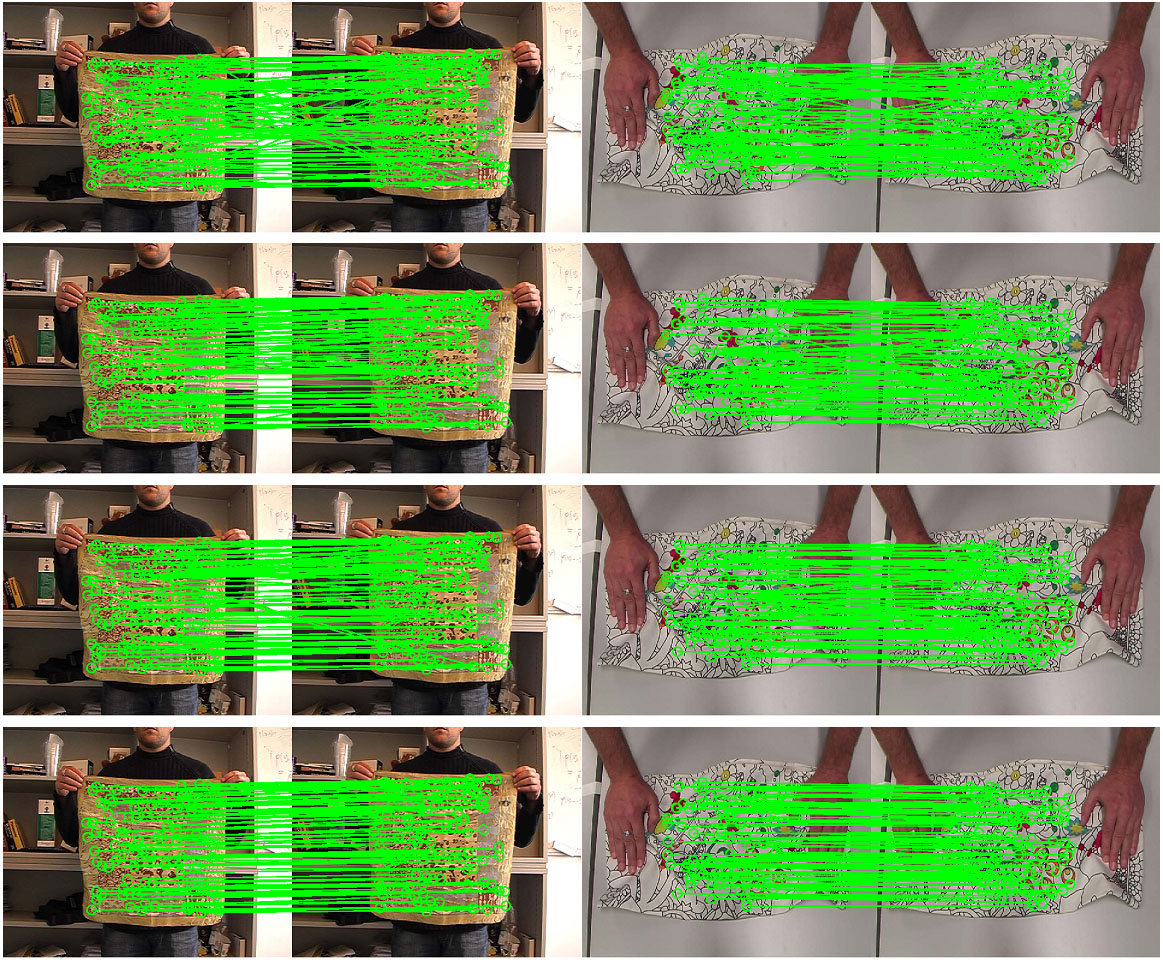
\includegraphics[width=1.00\linewidth]{figures/2DDeformable.jpg}
  \caption{Matching results. Left: cloth set, selected from frame 85 to 110, right: cushion set, selected from frames 144 to 213.
  Top to bottom, spectral method [Cour et al. 2006], hyper graph matching method [Zass and Shashua 2008], a Third-order tensor [Duchenne et al. 2009], and SuperMatching algorithm.}
\label{fig:2DDeformable}
\end{figure}

%----------------------------------------
%  deformable matching results TABLE
%----------------------------------------
\begin{table}
%\vspace{-4mm}
\centering
%\renewcommand{\arraystretch}{0.8}
\tabcolsep=1pt
\setlength{\aboverulesep}{0pt}
\setlength{\belowrulesep}{0pt}
\caption{Error rate of deformable surface matching.}
\hspace{-5ex}
\label{tab:errorrate1}
\small
\begin{tabular}{l|c c c c | c c c c | c c}
\toprule
{Dataset}  & \multicolumn{4}{|c|}{ {cloth}} & \multicolumn{4}{c|}{ {cushion}} & & \\
\hline
 {Matching frames} &  {F80-}	&  {F90-}	& {F95-}	& {F100-} & {F144-} & {F156-}	& {F165-}	& {F172-} & {Feature}	& {Time}  \\
 {}                &  {F90 }    &  {F95 }   & {F100}    & {F105}  & {F156}  & {F165}    & {F172}    & {F188}  & {Tuples}    &  {(s)} \\
\hline
 {SuperMatching}   &  {17\%}    &  {15\%}	& {16\%} 	& {19\%}  & {34\%}	& {40\%}	& {31\%}	& {44\%}  &  {20k}	    &  {8}  \\
%\hline
 {\cite{Zass08}}   & {27\%}	    & {21\%}	& {30\%}	& {28\%}  & {56\%}  & {61\%}    & {46\%}	& {57\%}   & {40k}	    & {6.5}  \\
%\hline
{\cite{Duchenne09}} & {33\%}    & {23\%}    & {27\%}	& {35\%}  & {61\%}	& {69\%}	& {53\%}	& {58\%}   & {1010k}    & {13}  \\
%\hline
 {\cite{Cour06}}   & {73\%}     & {71\%}	&  {78\%}	& {73\%}  & {86\%}  & {95\%}	& {72\%}	& {93\%}   & {--}       & {5}  \\
\bottomrule
\end{tabular}%
%\vspace{-27pt}
%\vspace{-8mm}
\end{table}%
%
%%%RRM This table would be much better if you showed the percentage of
%%%RRM CORRECT matches, not the percentage of ERRORS.

%-------------------------------------------------------------------------
\subsection{3D rigid shape scans}
\label{subsec:3DRigid}

Secondly, we used  SuperMatching to align multiple 3D rigid shape scans, as would
be done in building a complete model from a set of scans from different viewpoints.
For the multiple scans, the
third-order matching is first performed between two consecutive frames.
%%%RRM frames = scans?
Then rigid transforms can be computed from the three compatible matching feature points.
%%%RRM I dont understand the above. Once you have done matching
%%%RRM surely the best solution is to compute the transform by a least
%%%RRM squares fit to all matches, possibly with some robust least squares
%%%RRM method which can reject any outliers.
The transform which brings the most data points within a threshold of a point in the model is chosen as the optimal aligning transform~\cite{Huttenlocher90}.
%%%RRM This is too brief to really understand. Also, it is not clear how this
%%%RRM is related to the matched feature spoints
As discussed in~\cite{Gelfand05}, such a voting scheme is guaranteed to find the optimal alignment  between the pairwise scans and is independent of the initial pose of the input scans.
After the initial pairwise matching, the alignment is refined by the iterative closest point (ICP) algorithm following~\cite{Gelfand05}.
%%%RRM Why do you refine it? Is this because the feature points are only a
%%%RRM subset of all points? or some other reason?
Figure~\ref{fig:3DRigid} illustrates the approach.
Above, a sheep's head  is scanned from multiple viewpoints. Below, matching is used to align 10 scans which are then merged to produce a single  shape.
Pairs of consecutive scans are matched using the SuperMatching algorithm .

\begin{figure}
\centering
  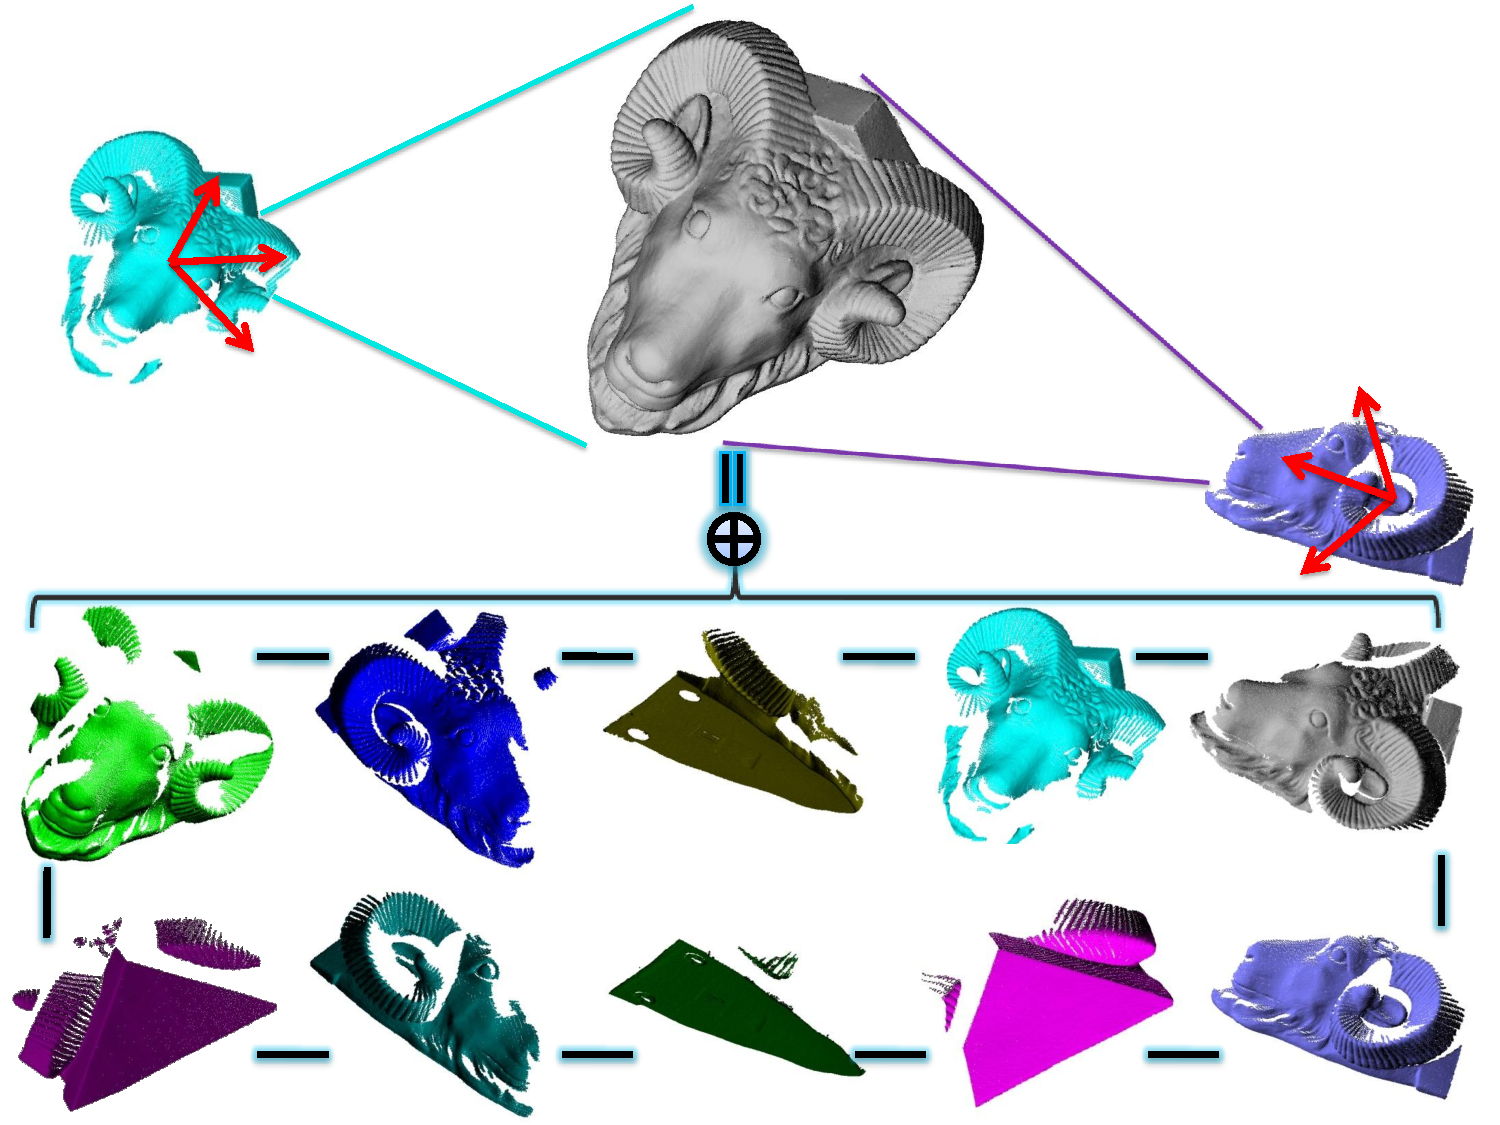
\includegraphics[width=0.99\linewidth]{figures/3DRigid.pdf}
  \caption{Alignment of several sheep head scans from different viewpoints. Above: scans are captured from different viewpoints. Below: the final shape is formed from 10 aligned scans.}
\label{fig:3DRigid}
\end{figure}

%%%RRM This experiment is just a demo. There is nothing here to
%%%RRM prove that the results are better than those from some other approach.
%%%RRM We need some way of showing our results are better by doing a comparison
%%%RRM with other methods.

%%%RRM Actually, there are some datasets out there with known transofrmations
%%%RRM between them. We could try to show we can estimate the transformations
%%%RRM more accurately than other methods.
%%%RRM See for example the dataset used in
%%%RRM http://ralph.cs.cf.ac.uk/papers/Geometry/crf.pdf

%-------------------------------------------------------------------------
\subsection{3D articulated shape synthetic data}
\label{subsec:3darticulated}

Thirdly, we present another application, registration of (approximately) articulated shapes. Such problems are common in dynamic range scanning.
Given a sequence of range scans of a moving articulated subject, our method automatically registers all data to produce a complete 3D shape.
Note that, unlike many other methods, our method does not need any of manual segmentation, user specified markers, or a prior template.
While the problem of non-rigid registration of deformable shapes is ill-posed and no algorithm is applicable to all scenarios, 
we believe that our approach pushes the limits of what can be achieved with minimal prior information, and is robust to partial data with holes.

Articulated registration is performed in two main steps.
We first precompute an initial pairwise registration for each pair of consecutive frames, then perform articulated shape reconstruction as in~\cite{Pekelny08}.
Although the partial scans have missing data and their poses are different,  SuperMatching still produces accurate matching.
Correspondences between slippage feature points are established by  SuperMatching; these permit robust registration of scans  by computing piecewise rigid transformations.
These transformations are propagated from the slippage feature points to the entire set of points in each scan using nearest neighbor interpolation.
%%%RRM This may not work well near joints
Segmentation of  the scans into rigid parts can readily be done by clustering the transformations obtained from the slippage feature points, using the mean shift algorithm~\cite{Comaniciu02}.
This information is used as the input to the second step of articulated shape reconstruction following~\cite{Pekelny08};
this algorithm identifies and tracks the rigid parts in each frame, while accumulating  geometric information over time.
However,~\cite{Pekelny08} requires the user to manually segment each range scan in advance,  whereas we automatically determine  the segmentation.

Figure~\ref{fig:3DHand} shows an articulated hand example.
This synthetic data is generated from a deformation sequence, and the final registered shape is produced from these partial data. Note that this data contains just a single
view in each frame, and does not contain a complete object, which makes the problem
more challenging.
%%%RRM I added the above sentence - check it (and caption of Fiig 4)
By using synthetic data, we are able to evaluate the robustness of our reconstruction method using the ground truth, as shown below in Figure~\ref{fig:3DHand}.
Quantitatively, we measured the maximum of the average distance of the reconstruction over all frames as $0.001 D$ where $D$ is the bounding box diagonal length, and
the greatest distance error in any one frame was  $0.012 D$.

\begin{figure}
\centering
  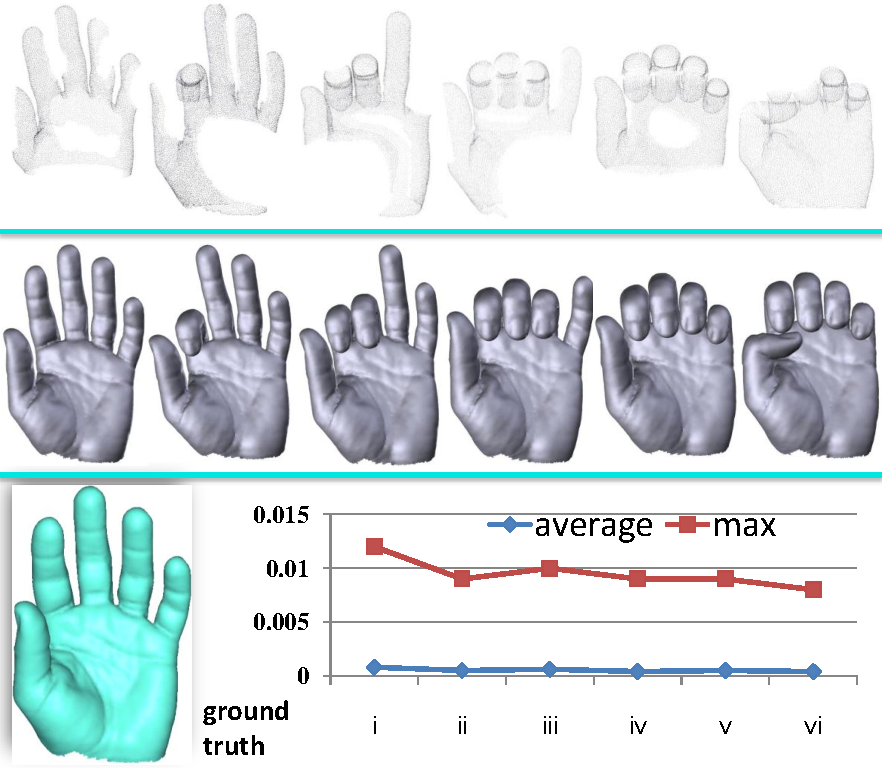
\includegraphics[width=0.99\linewidth]{figures/3DHand.pdf}
  \caption{The registration of articulated hand.
  Above: single view per frame synthetic data  is generated from a deformation sequence. Correspondences, transforms, and segmentation are deduced (center).
  %%%RRM Not clear what the yellow parts are, and why they are on different fingers.
  %%%RRM Why not show the segmentation in each frame?
  Below: ground truth shape, and average and maximum distance from the ground truth per frame.}
\label{fig:3DHand}
\end{figure}

%-------------------------------------------------------------------------
\subsection{3D depth scans with colour information}
\label{subsec:3dColored}

Complementary to the evaluation presented above,
we also provide a real-world example demonstration of SuperMatching. In this case,
real world data with surface color information was captured using a Kinect camera~\cite{Kinect12}, and both SIFT and slippage features were used as a basis for SuperMatching, 
which resulted in robust matches without significant outliers, as illustrated in Figure~\ref{fig:3DReal}.
%%%RRM Again, this is just a demo, without an numerical results.
%%%RRM Also, you do not say enough about what you did for someone to reproduce this
\begin{figure}
\centering
  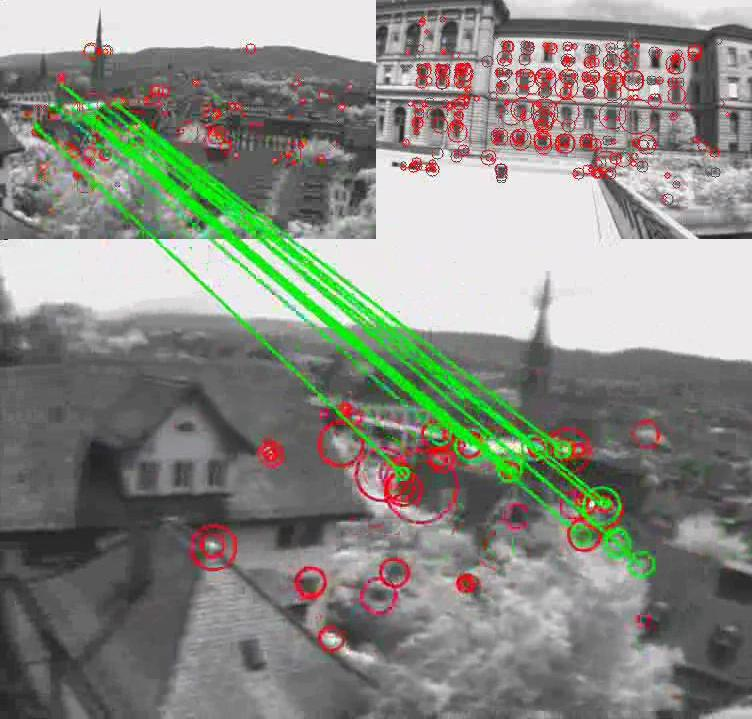
\includegraphics[width=0.98\linewidth]{figures/3DReal.jpg}
  \caption{3D real depth scans with color information, captured using Kinect.
  Above: two given different local pre-scans.  Below: a single scan.
  Matching points are connected by  green lines.}
\label{fig:3DReal}
%%%RRM I dont really understand this result. I though the kinect scanned
%%%RRM nearby objects yet this shows pictures of trees and buildings a long distance away
%%%RRM Also, I dont see the point of the top right image here. It shows nothing
%%%RRM about matching.
\end{figure}
